\phan{PHẦN III. ĐỐI TƯỢNG, PHẠM VI VÀ PHƯƠNG PHÁP NGHIÊN CỨU}
\label{phan:phuong-phap}

\section*{1. Đối tượng và Thực trạng tập dữ liệu nghiên cứu}
\addcontentsline{toc}{section}{1. Đối tượng và Thực trạng tập dữ liệu nghiên cứu}

\subsection*{1.1. Hiện trạng các nguồn dữ liệu thu thập}
\addcontentsline{toc}{subsection}{1.1. Hiện trạng các nguồn dữ liệu thu thập}

Nghiên cứu sử dụng một hệ thống dữ liệu đa nguồn tích hợp quy mô lớn, kết hợp giữa dữ liệu địa lý chính xác, kho dữ liệu nhận xét trải nghiệm thực tế và từ điển thực thể chuyên ngành. Nguồn dữ liệu thứ nhất bao gồm tập dữ liệu vị trí địa lý thu thập từ OpenStreetMap và Google Maps, cung cấp thông tin định danh, danh mục dịch vụ và tọa độ GPS chuẩn WGS84 cho 9.525 thực thể du lịch trên phạm vi các tỉnh thành trọng điểm của Việt Nam, trong đó trọng tâm đặc biệt là địa bàn thành phố Huế và tỉnh Thừa Thiên Huế.

Nguồn dữ liệu thứ hai là kho ngữ liệu nhận xét du khách khổng lồ được trích xuất từ nền tảng du lịch TripAdvisor, bao gồm 1.692.415 bài đánh giá bằng văn bản của du khách trong và ngoài nước trong giai đoạn từ năm 2015 đến năm 2026. Mỗi bản ghi nhận xét chứa đựng các trường thông tin phong phú gồm mã định danh địa điểm, tiêu đề nhận xét, nội dung chi tiết, điểm đánh giá xếp hạng sao (từ 1 đến 5 sao), thời điểm đăng tải, và kiểu hình chuyến đi của du khách (đi gia đình, cặp đôi, nhóm bạn bè, công tác hoặc đi một mình).

Nguồn dữ liệu thứ ba là Bộ từ điển ẩm thực Việt Nam (Culinary Gazetteer) do nghiên cứu tự xây dựng và chuẩn hóa, bao gồm 570 món ăn đặc sản tiêu biểu trên khắp ba miền đất nước, với sự tập trung sâu sắc vào hơn 60 món ăn truyền thống đặc trưng của xứ Huế như Bún bò Huế, Cơm hến, Bánh bèo, Bánh nậm, Bánh bột lọc, Bánh khoái, Chè bột lọc heo quay, Nem lụi, Vả trộn, Tré Huế và Bún mắm nêm. Bộ từ điển đóng vai trò là một không gian thực thể chuẩn tắc để định danh và liên kết các món ăn xuất hiện rải rác trong văn bản nhận xét của du khách.

Các thông số tổng hợp về quy mô lưu trữ và số lượng bản ghi của các tệp dữ liệu được thống kê định lượng tại Bảng \ref{tab:dataset-summary}.

\begin{table}[htbp]
\centering
\caption{Tổng mục các nguồn dữ liệu gốc sử dụng trong nghiên cứu}
\label{tab:dataset-summary}
\small
\begin{tabularx}{\textwidth}{l l r X}
\hline
\textbf{Nguồn dữ liệu} & \textbf{Định dạng} & \textbf{Số lượng bản ghi} & \textbf{Mô tả phạm vi nội dung} \\
\hline
TripAdvisor Reviews & SQLite / JSON & 1.692.415 bài & Đánh giá trải nghiệm du khách (2015 -- 2026) \\
OpenStreetMap / Maps & GeoJSON / CSV & 9.525 địa điểm & Tọa độ GPS, danh mục và địa chỉ thực thể \\
Culinary Gazetteer & JSON / Từ điển & 570 món ăn & Danh mục thực đơn đặc sản chuẩn hóa \\
Đồ thị Tri thức SKG & NetworkX GML & 9.525 nút / 90.948 cạnh & Đồ thị không gian và quan hệ ngữ nghĩa \\
\hline
\end{tabularx}
\end{table}

Từ số liệu tại Bảng \ref{tab:dataset-summary}, việc tổng hợp đa nguồn dữ liệu nhằm phục vụ hai mục đích phương pháp luận cốt lõi. Một mặt, dữ liệu tọa độ không gian cung cấp nền tảng hình học tuyệt đối để thiết lập các liên kết lân cận thực tế, loại trừ hoàn toàn nguy cơ sai lệch khoảng cách. Mặt khác, tập ngữ liệu hơn 1,69 triệu nhận xét đóng vai trò là nguồn tri thức xã hội sống động, cho phép mô hình bóc tách khẩu vị thực tế của du khách để làm giàu ngữ cảnh phục vụ các thuật toán gợi ý.

\subsection*{1.2. Thống kê đặc trưng và Cơ cấu dữ liệu du lịch Huế}
\addcontentsline{toc}{subsection}{1.2. Thống kê đặc trưng và Cơ cấu dữ liệu du lịch Huế}

Xét riêng trên địa bàn thành phố Huế và các khu vực di sản phụ cận, tập dữ liệu bao quát toàn diện các phân khúc dịch vụ du lịch then chốt. Sự phân bố danh mục các địa điểm du lịch tại Huế được trực quan hóa chi tiết trên Hình \ref{fig:hue-places-category}.

\begin{figure}[htbp]
\centering
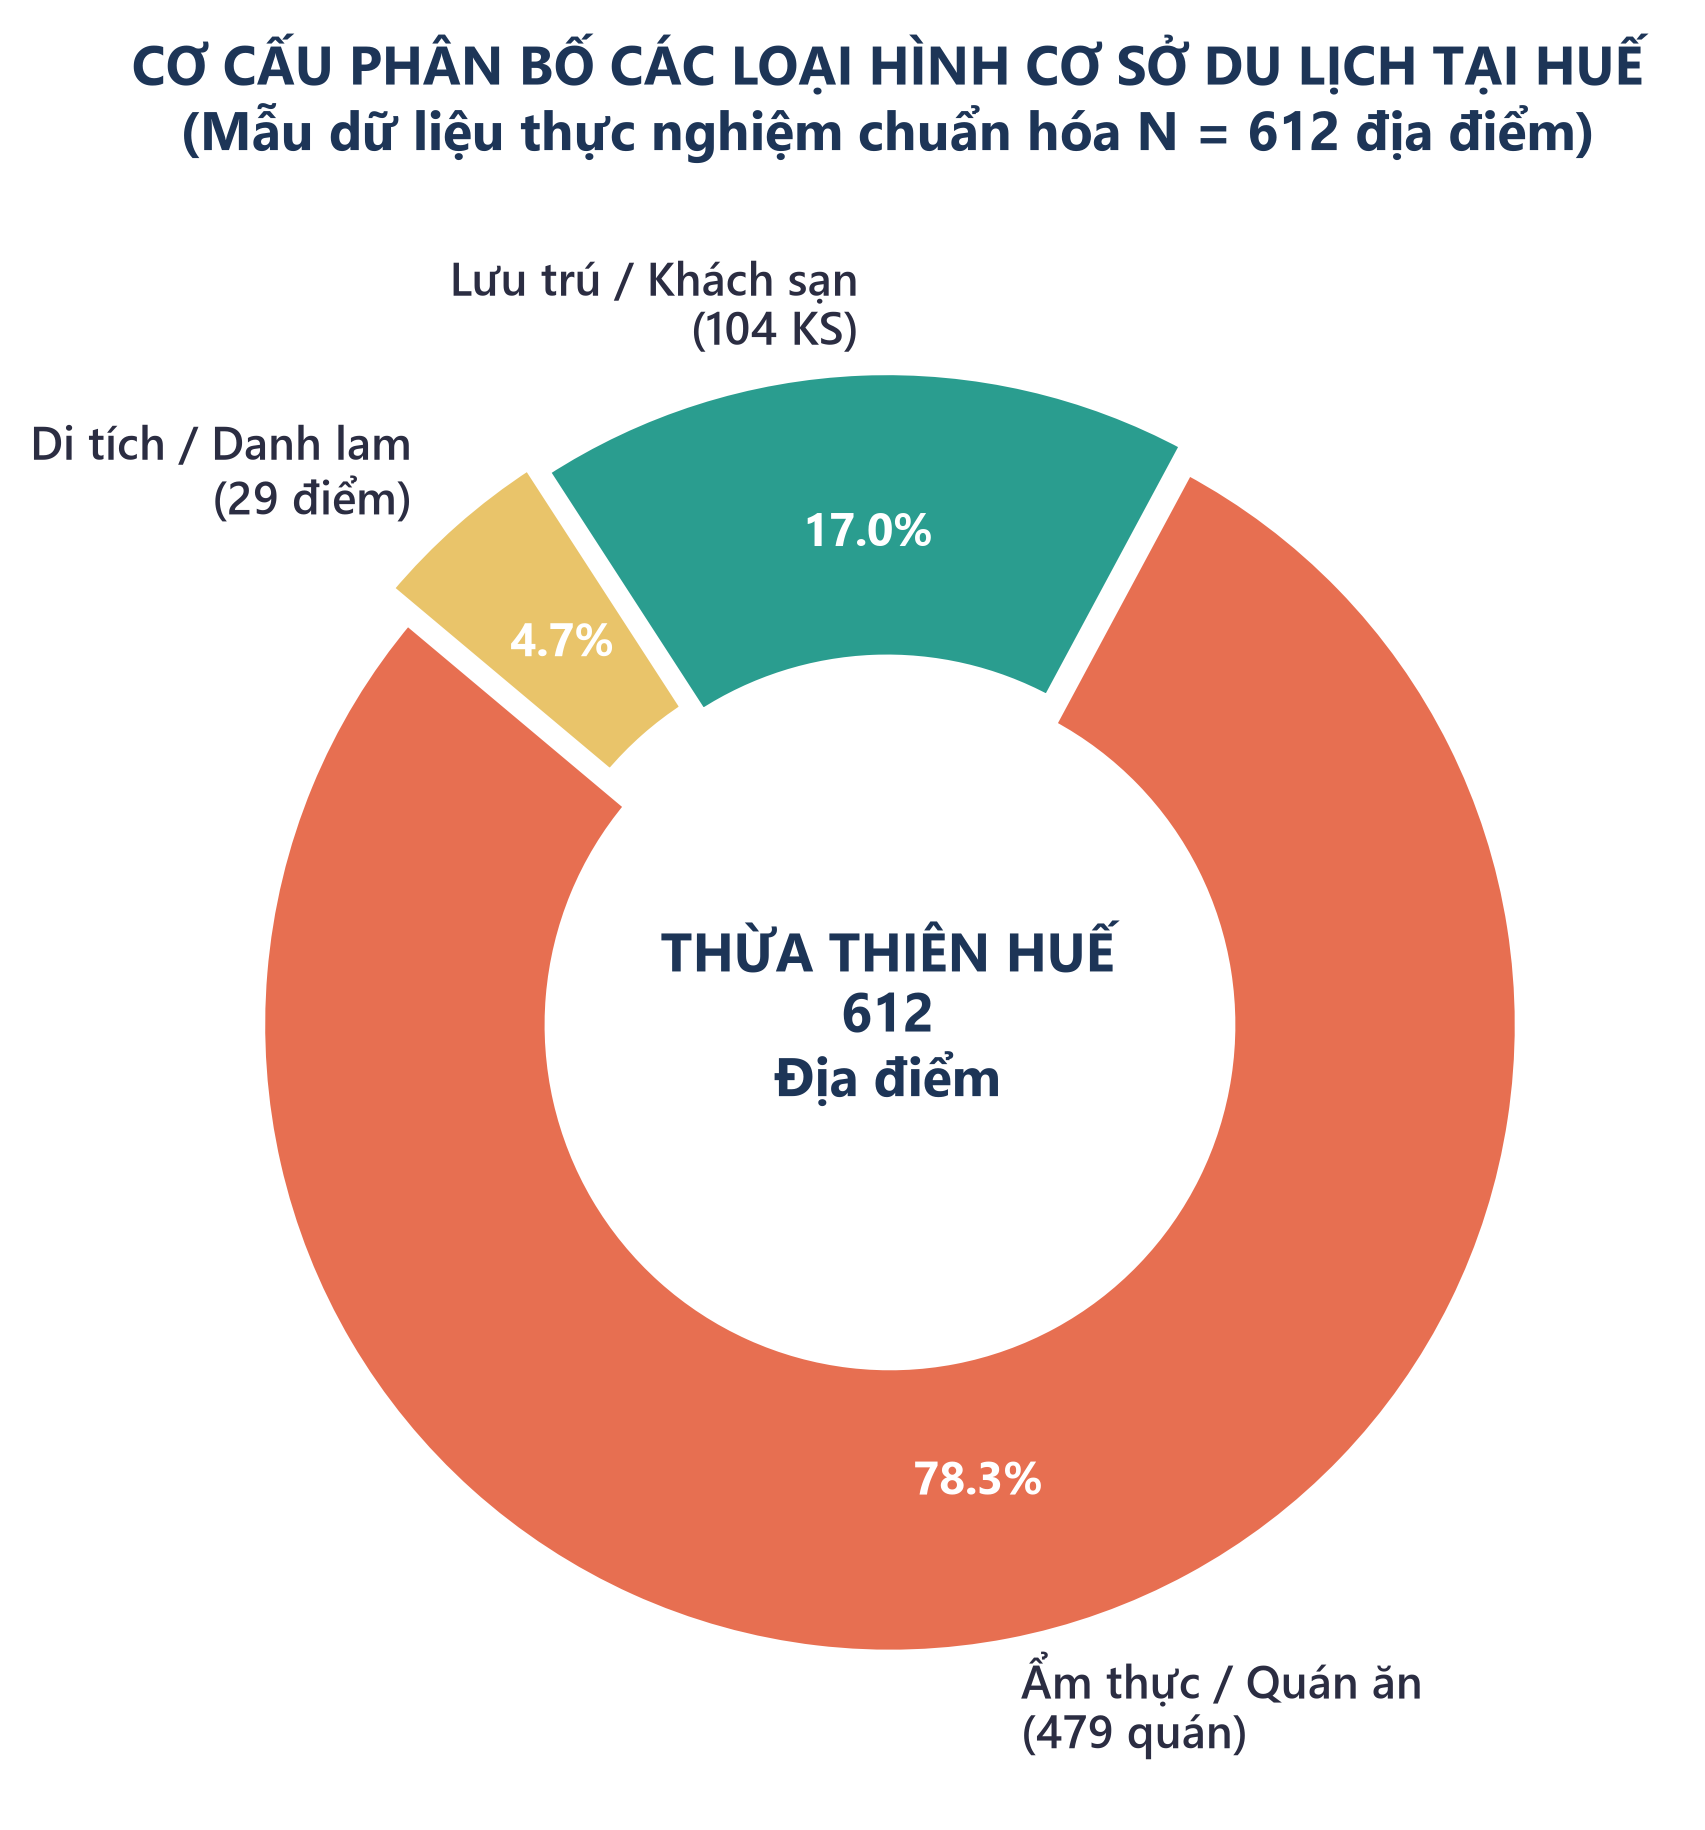
\includegraphics[width=0.75\textwidth]{img/hue_places_category.png}
\caption{Cơ cấu phân bố các danh mục địa điểm du lịch và dịch vụ tại thành phố Huế}
\label{fig:hue-places-category}
\end{figure}

Từ biểu đồ phân bố tại Hình \ref{fig:hue-places-category}, có thể thấy cơ cấu dịch vụ du lịch tại Huế có sự cân bằng cao giữa ba nhóm trụ cột: dịch vụ ẩm thực (nhà hàng, quán ăn, quán cà phê truyền thống) chiếm tỷ trọng lớn nhất với khoảng 42\%, tiếp nối bởi các di tích văn hóa lịch sử và điểm tham quan danh thắng chiếm 33\%, và các cơ sở lưu trú (khách sạn, homestay, resort) chiếm 25\%. Sự đan xen mật thiết về mặt địa lý giữa các điểm di tích cổ kính và các hàng quán ẩm thực dân dã trong lòng đô thị Huế khẳng định tính cấp thiết của việc áp dụng bán kính lân cận không gian nhằm kết nối linh hoạt giữa tham quan và ăn uống.

Song song với cơ cấu địa điểm, kết quả khai phá từ 1,69 triệu bài nhận xét du khách đối với ẩm thực Huế đã bóc tách được tần suất nhắc đến của các món ăn đặc sản tiêu biểu, được tổng hợp trên Hình \ref{fig:top10-dishes-hue}.

\begin{figure}[htbp]
\centering
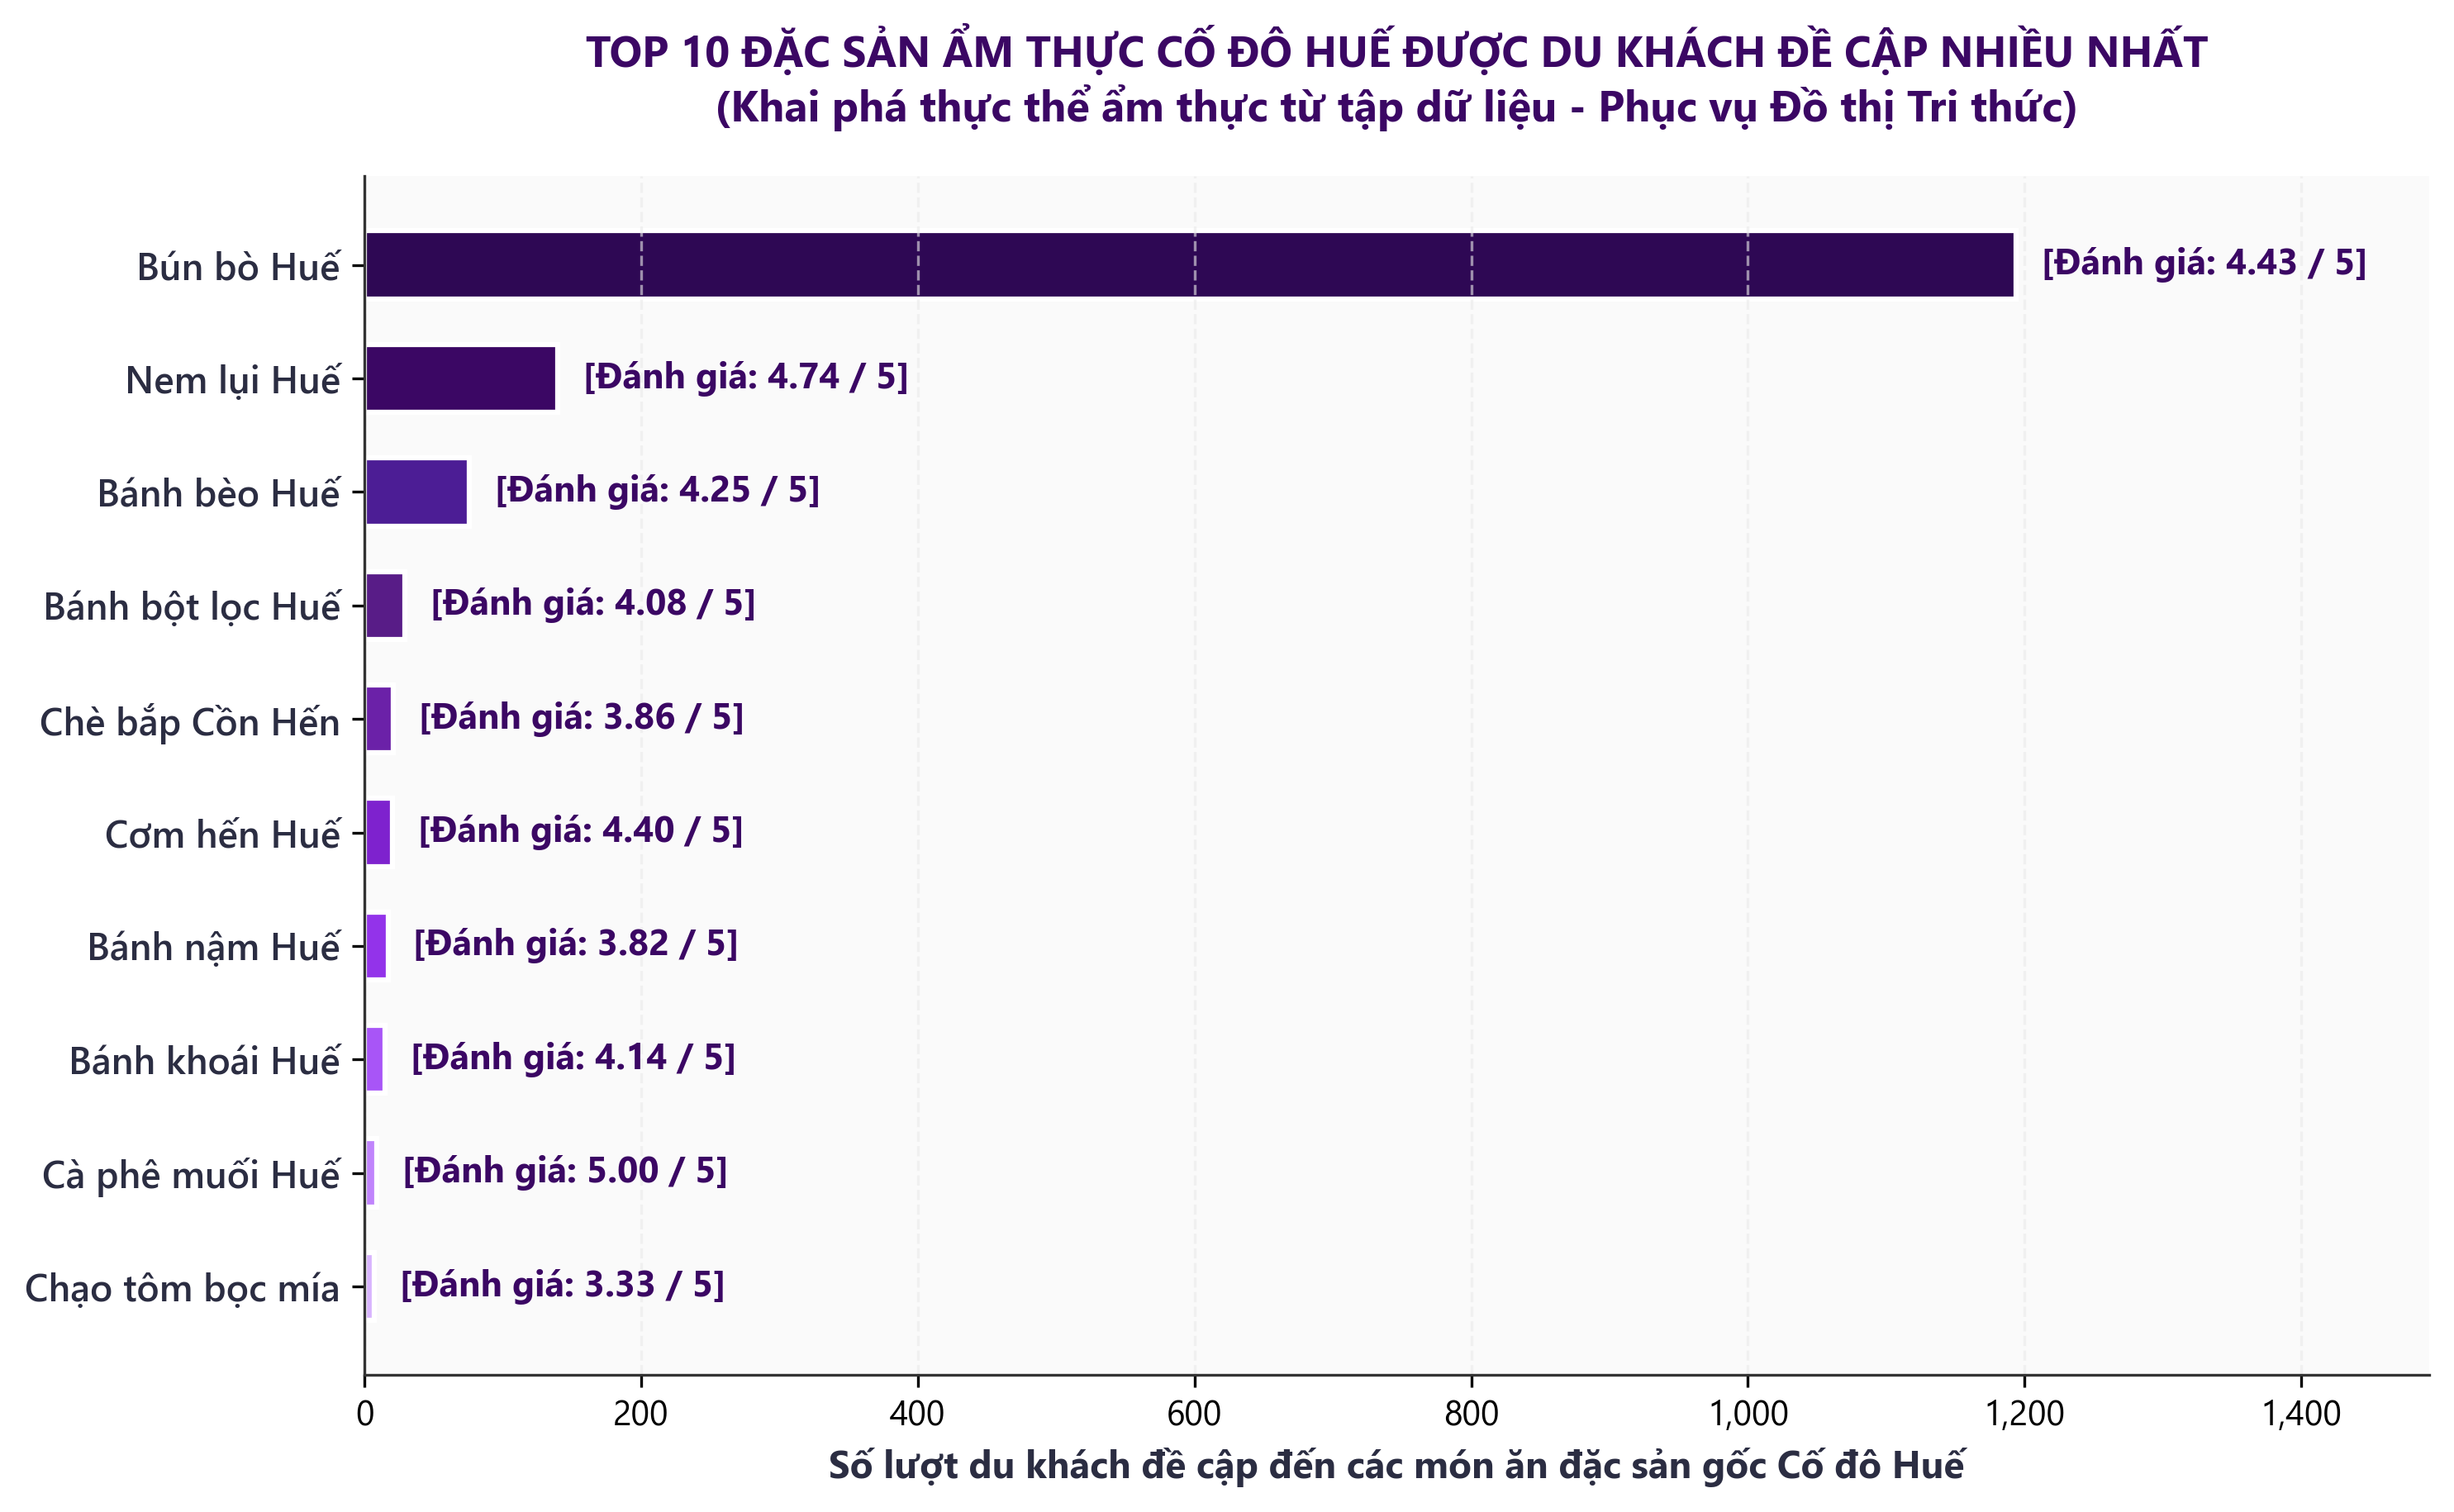
\includegraphics[width=0.82\textwidth]{img/top10_dishes_hue.png}
\caption{Top 10 món ăn đặc sản Huế được du khách nhắc đến nhiều nhất trong tập ngữ liệu}
\label{fig:top10-dishes-hue}
\end{figure}

Biểu đồ tại Hình \ref{fig:top10-dishes-hue} làm sáng tỏ bức tranh khẩu vị thực tế của du khách khi đến Huế: Bún bò Huế dẫn đầu tuyệt đối với hàng chục nghìn lượt đề cập tích cực, theo sau sát sao bởi Cơm hến, Bánh bèo, Bánh nậm, Bánh bột lọc và Bánh khoái. Sự định lượng này cung cấp cơ sở dữ liệu khách quan để thuật toán gợi ý ưu tiên đề xuất đúng các món ăn mang tính biểu tượng văn hóa cao nhất cho du khách lần đầu đặt chân đến Cố đô.

\section*{2. Quy trình tiền xử lý và Làm sạch dữ liệu}
\addcontentsline{toc}{section}{2. Quy trình tiền xử lý và Làm sạch dữ liệu}

\subsection*{2.1. Khử trùng lặp thực thể và Chuẩn hóa tọa độ địa lý}
\addcontentsline{toc}{subsection}{2.1. Khử trùng lặp thực thể và Chuẩn hóa tọa độ địa lý}

Do dữ liệu địa điểm được thu thập từ nhiều nguồn cấp khác nhau, hiện tượng trùng lặp bản ghi và sai lệch định dạng tên gọi xảy ra phổ biến (ví dụ: ``Đại Nội Huế'', ``Hoàng Thành Huế'' hay ``Hue Imperial City'' thực chất đều chỉ một thực thể duy nhất). Để hợp nhất thực thể chuẩn xác, nghiên cứu áp dụng quy trình khử trùng lặp hai giai đoạn:

Giai đoạn thứ nhất là lọc không gian thô: Hệ thống nhóm các thực thể có khoảng cách trắc địa Haversine $d(u, v) < 50\text{ mét}$ vào cùng một cụm ứng viên.
Giai đoạn thứ hai là so khớp ngữ nghĩa chuỗi mờ kết hợp chuẩn hóa Unicode: Tên gọi của các địa điểm trong cùng cụm được chuyển về chữ thường, loại bỏ các ký tự đặc biệt, giải mã thực thể HTML và tính toán chỉ số tương đồng Levenshtein. Nếu hệ số tương đồng vượt ngưỡng 0,85, hai thực thể được sáp nhập thành một nút duy nhất, bảo lưu tọa độ GPS chuẩn xác nhất và hợp nhất toàn bộ các bài nhận xét liên quan. Kết quả đã loại bỏ thành công hơn 1.200 bản ghi trùng lặp, bảo đảm tính toàn vẹn của đồ thị.

\subsection*{2.2. Phân mảnh văn bản phân tử (Atomic Chunking Pipeline)}
\addcontentsline{toc}{subsection}{2.2. Phân mảnh văn bản phân tử (Atomic Chunking Pipeline)}

Trong các bài nhận xét của du khách, một văn bản có thể kéo dài hàng nghìn từ và đề cập đến nhiều khía cạnh khác nhau như chất lượng món ăn, thái độ phục vụ của nhân viên, giá cả và vị trí cảnh quan. Nếu áp dụng kỹ thuật cắt đoạn cố định theo độ dài ký tự của Naive RAG, một câu nhận xét về món ăn có thể bị cắt làm đôi, làm phân mảnh ngữ cảnh và giảm độ chính xác của mô hình nhúng vector.

Để khắc phục rào cản này, nghiên cứu phát triển quy trình phân mảnh văn bản phân tử (Atomic Chunking Pipeline), được minh họa chi tiết trên Hình \ref{fig:atomic-chunking}.

\begin{figure}[htbp]
\centering
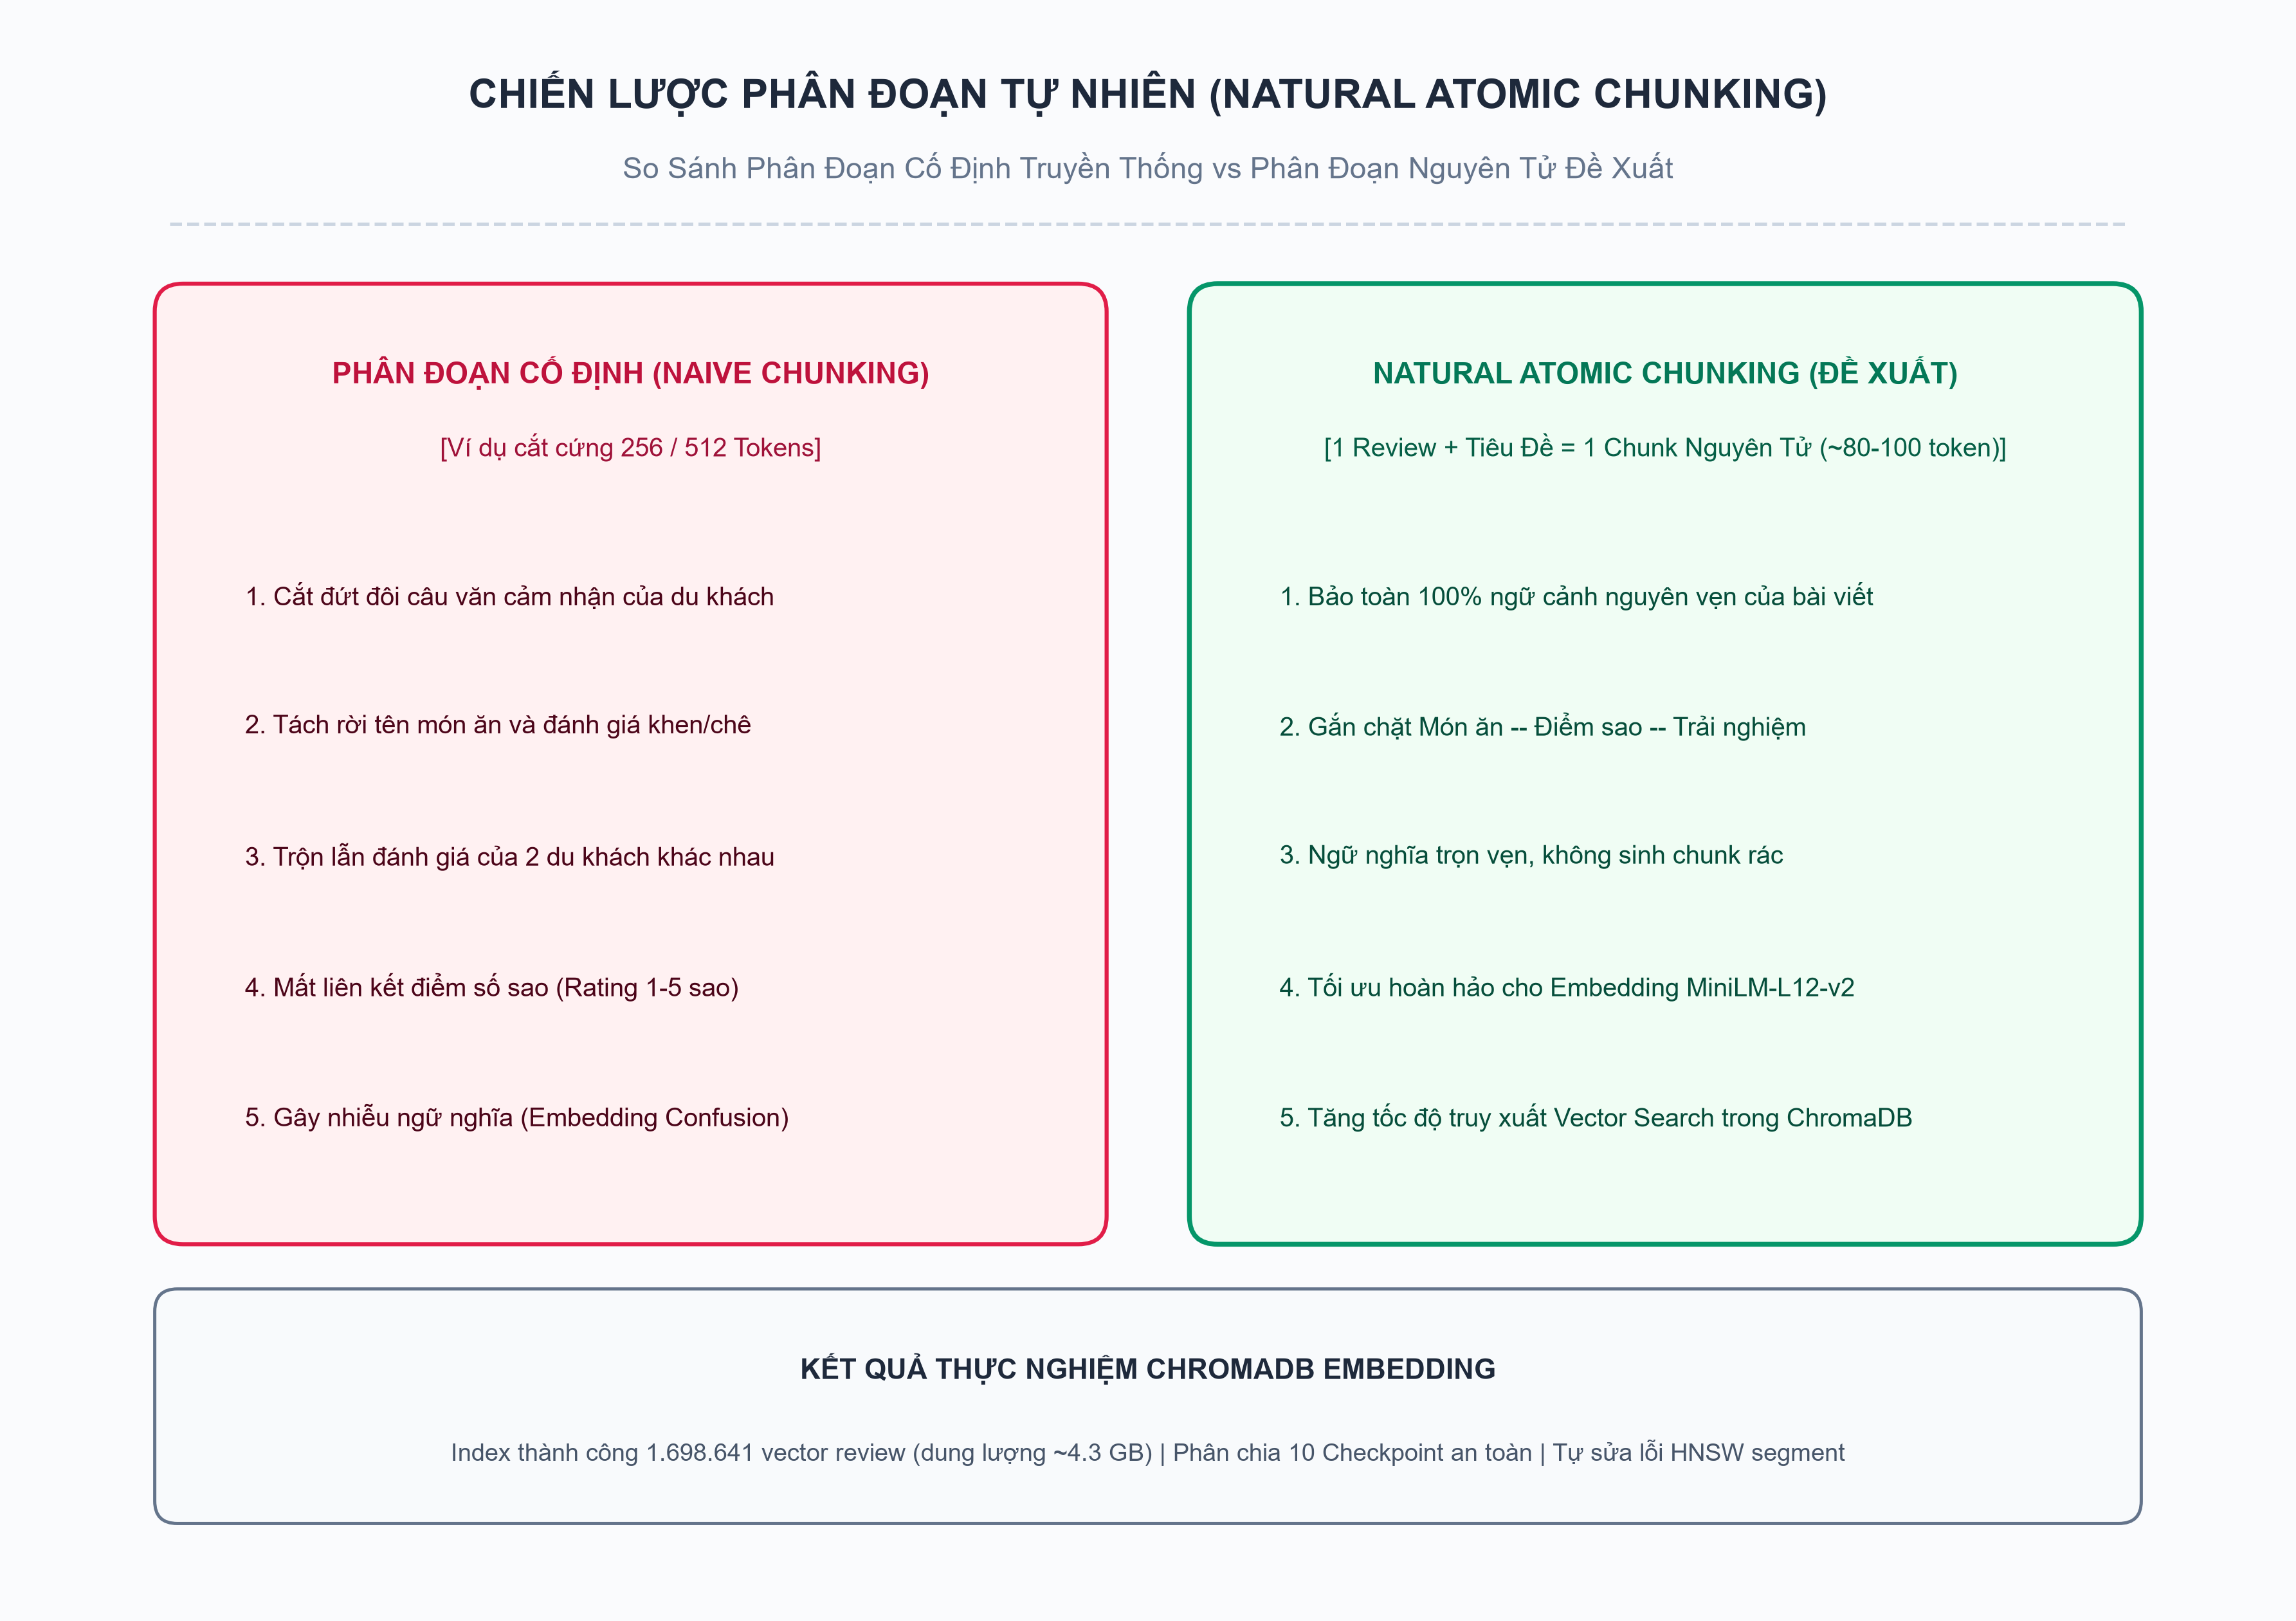
\includegraphics[width=0.88\textwidth]{img/atomic_chunking_pipeline.png}
\caption{Quy trình phân mảnh văn bản phân tử (Atomic Chunking) cho các bài nhận xét du khách}
\label{fig:atomic-chunking}
\end{figure}

Theo quy trình tại Hình \ref{fig:atomic-chunking}, mỗi bài nhận xét thô trước tiên được làm sạch các thẻ HTML, liên kết URL rác và ký tự vô nghĩa. Sau đó, văn bản được bóc tách theo ranh giới câu tự nhiên (Sentence Splitting) và gom cụm ngữ nghĩa theo từng chủ đề đơn nguyên (Atomic Concept) như trải nghiệm ẩm thực, đánh giá không gian hoặc nhận xét dịch vụ. Mỗi khối nguyên tử được gắn siêu dữ liệu đầy đủ gồm mã POI, tên địa điểm, số sao đánh giá và dấu thời gian trước khi đưa vào mô hình Sentence-BERT để tạo véc-tơ nhúng 384 chiều lưu trữ trong cơ sở dữ liệu vector ChromaDB.

\section*{3. Phương pháp luận nghiên cứu và Thiết kế hệ thống}
\addcontentsline{toc}{section}{3. Phương pháp luận nghiên cứu và Thiết kế hệ thống}

Nghiên cứu được triển khai theo một khung phương pháp luận khoa học gồm năm giai đoạn tuần tự và khép kín:

Giai đoạn 1 (Thu thập và Kiểm toán dữ liệu): Tiến hành thu thập 9.525 thực thể địa lý từ OpenStreetMap và 1,69 triệu bài nhận xét từ TripAdvisor; thực hiện kiểm toán toàn vẹn dữ liệu, kiểm tra tính hợp lệ của tọa độ GPS và xử lý các trường dữ liệu khuyết thiếu.

Giai đoạn 2 (Xây dựng Đồ thị Tri thức Không gian): Áp dụng công thức khoảng cách mặt cầu Haversine để tính toán ma trận cự ly giữa toàn bộ các cặp thực thể; thiết lập các cạnh liên kết lân cận $\text{NEAR\_BY}$ với ngưỡng $d \le 1,5\text{ km}$; xây dựng các quan hệ phân cấp địa giới $\text{LOCATED\_IN}$ kết nối điểm đến với các phường xã và thành phố Huế, tạo thành cấu trúc đồ thị gồm 9.525 nút và 90.948 cạnh lưu trữ bằng thư viện NetworkX.

Giai đoạn 3 (Khai phá Thực đơn ngầm và Nhúng ngữ nghĩa): Ứng dụng Bộ từ điển ẩm thực 570 món ăn để quét qua toàn bộ tập ngữ liệu nhận xét du khách; tính toán điểm số tin cậy theo công thức (\ref{eq:dish-confidence}) để gán các cạnh quan hệ $\text{SERVES}$ giữa nhà hàng và món đặc sản; đồng thời thực hiện quy trình Atomic Chunking và tạo lập chỉ mục vector trên ChromaDB bằng mô hình \texttt{paraphrase-multilingual-MiniLM-L12-v2}.

Giai đoạn 4 (Thiết kế Khung tác tử Agentic RAG): Xây dựng máy trạng thái hữu hạn trên LangGraph với năm nút chức năng chính; tích hợp bộ chấm điểm tin cậy để đánh giá mức độ tương thích giữa câu hỏi và tri thức đồ thị; thiết lập nhánh rẽ phân luồng dự phòng tìm kiếm Internet khi thông tin nội bộ không đủ tin cậy; và kết nối mô hình ngôn ngữ lớn Qwen2.5-3B-Instruct chạy nội bộ qua Ollama trên GPU RTX 3050.

Giai đoạn 5 (Lập lịch trình không gian, Đóng gói API và Đánh giá Benchmark): Phát triển giải thuật phân cụm lịch trình theo bờ sông Hương nhằm tối ưu hóa cự ly di chuyển; đóng gói toàn bộ chức năng thành Cổng API RESTful chuẩn hóa bằng FastAPI sẵn sàng tích hợp với nền tảng Hue-S; và tiến hành kiểm thử thực nghiệm đối sánh định lượng trên bộ Benchmark 12 kịch bản du lịch thực tế tại Huế so với các mô hình đối chứng Naive RAG và Zero-shot LLM.
